\chapter{Problema 3}

\section{Descripción del problema}
Un videojuego se juega por turnos y se representa en un mapa cuadriculado bidimensional
de f filas y c columnas. El jugador siempre entra al mapa por la esquina superior derecha,
y sale por la esquina inferior izquierda. En cada turno, los posibles movimientos del
jugador son: ir 1 casilla a la izquierda, ir 1 casilla abajo, o moverse 1 posición a la casilla
inferior izquierda. Cada casilla del mapa puede estar vacía, contener un muro, o contener
una bolsa de oro. Todas las casillas son transitables salvo las que tienen muros. El objetivo
consiste en llegar a la salida pudiendo recoger tanto oro como sea posible (pasar por tantas
casillas que contengan una bolsa como se pueda). En el ejemplo siguiente, el jugador
puede conseguir un máximo de 3 bolsas de oro con los movimientos permitidos.

\begin{figure}[h]
    \centering
    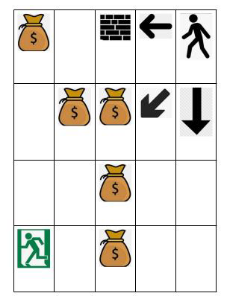
\includegraphics[width=0.4\linewidth]{figures//problema3/imagen.png}
    \label{fig:enter-label}
\end{figure}

\section{Solución: Diseño de componentes y del algoritmo}


\subsection{Resolución del problema por etapas}

Este problema puede resolverse mediante etapas. En cada etapa podemos barajar que posibilidad nos sale más rentable acorde a nuestros objetivos. Como nuestros objetivos son maximizar la cantidad de oro que vamos recogiendo en función de las casillas por las que pasamos, debemos de escoger aquellas posiciones, que en cómputo total, al salir del mapa del juego consigamos la máxima cantidad de bolsas de oro. Cabe destacar que para las explicaciones que vamos a realizar a continuación vamos a pensar que la representación del mapa va a corresponder con una matriz.

\subsection{Ecuación recurrente}

La solución depende de las etapas (a que posición debo de mover el personaje del videojuego para obtener la mayor cantidad de oro). Vamos a denotar como $T(i,j)$ el máximo número de bolsas de oro que se puede conseguir al llegar a la casilla $(i,j)$. Como sabemos \textit{i} y \textit{j} corresponde con las posiciones dentro de nuestro mapa del videojuego.

Debemos de considerar el tipo de casilla, ya que puede ser casilla con muro, sin muro, y dentro de sin muro que haya oro o no. Lo que haremos será denotar a las casillas con un valor negativo muy grande, es decir, casillas = \(-\infty\). Para inicializar toda la matriz, y ya mediante el algoritmo de programación dinámica vamos a ir resolviendo el problema y devolver una matriz final T, la cual explicaremos a continuación. 
Por lo que podemos afirmar que si la casilla \textit{(i,j)} tiene un muro $T(i,j)$ = \(-\infty\). Esto lo ampliamos a que valdrá $T(i,j)$ = \(-\infty\) cuando, en general, la casilla sea no transitable. También el valor puede llegar a ser no accesible debido a la propagación de la innaccibilidad. Al calcular los valores de \textit{T(i)(j)}, si todos los caminos posibles hacia una celda provienen de celdas inaccesibles (es decir, que contienen \textit{INT\_MIN}), entonces esa celda también será inaccesible. De esta manera, la inaccessibilidad se propaga correctamente a través de la matriz. Esta representación ayuda a asegurar que las celdas inalcanzables no se utilicen en cálculos posteriores.

En el caso de que no sea un muro, podemos establecer el valor de $T(i,j)$ en función de que si hay oro o no en la casilla. Así que podemos expresar $T(i,j)$ cuando no hay un muro de la siguiente manera:

\[T(i,j) = max \{T(i-1,j-1),T(i-1,j),T(i,j-1) + Oro(i,j)\} \]

Cabe destacar que va a variar en función de la posición en la que nos encontremos, ya que en el caso de que \textit{(i,j)} sea \textit{(0,0)} no se pueden acceder a diversas posiciones. La función \textit{Oro(i,j)} devuelve \textit{1} en el caso de que si haya oro en la casilla \textit{(i,j)} y \textit{0} en caso contrario.

En base a este planteamiento, podemos establecer que nuestra ecuación de recurrencia sería:

\[
T(i, j)  \begin{cases} 
T(i,j) = -\infty\ \text{   si hay un muro en (i,j) o es una casilla no transitable} \\
T(i,j) = max \{T(i-1,j-1),T(i-1,j),T(i,j-1) + Oro(i,j)\} \text{  si no hay muro en (i,j)}
\end{cases}
\]

Los casos base para esta ecuación serían: 

\begin{itemize}
    \item Si nos encontramos en la casilla inicial estamos en $T(0,0) = Oro (0,0)$. El valor depende si hay oro o no en la casilla inicial.
    \item Si nos encontramos una casilla se encuentra fuera del mapa o que posee un muro, se considera una casilla no transitable.
\end{itemize}

\subsection{Valor objetivo}

Se desea conocer $T(i,j)$, el valor máximo de bolsas de oro que se pueden conseguir transitando desde la casilla \textit{(0,0)} hasta la casilla (n-1,m-1) teniendo la posibilidad de moverse a las casillas \textit{(i-1,j-1), (i-1,j) y (i,j-1)}, podemos acceder a esas posiciones siempre y cuando \( i \in {0..n-1} \) y \( j \in {0..m-1} \)

\subsection{Verificación del cumplimiento del P.O.B}
En este caso siempre estamos calculando la solución óptima ya que la optimalidad de la casilla de \textit{(i,j)} se ha calculado en base a otros casos que a su vez también son óptimos, por lo que podemos concluir que también es óptimo. Básicamente, Cualquier solución óptima debe estar formada por subsoluciones óptimas. En este caso se cumple, dado que \textit{T(i,j)}, que asumimos óptimo, podrá tener valores \textit{T(i-1,j-1), T(i-1,j) o T(i,j-1)}. Estos valores también son óptimos, dado que la ecuación recurrente siempre va escogiendo el máximo entre los valores mencionados anteriormente. No es posible que exista un valor mayor que el máximo entre los valores para \textit{T(i,j).}

\subsection{Diseño de la memoria}
\begin{itemize}
    \item Para resolver el problema, usaremos una matriz, por lo que, \textit{T (i,j)} se representará como una matriz.
    \item Esta matriz tendrá n filas y m columnas, que estarán asociadas a el lugar correspondiente dentro del mapa. Únicamente, podrán optar por valores entre {0...n-1}.
    \item Cada celda de la matriz \textit{T(i,j)} contendrá el máximo valor de bolsas de oro que se pueden obtener hasta llegar a la casilla \textit{(i,j)} del mapa teniendo en cuenta los movimientos disponibles que se exponen en el problema.
    \item La manera en la que se va a ir rellenando la memoria (matriz) corresponde con ir asignando el correspondiente valor \textit{T(i,j)} a cada casilla de la matriz.
\end{itemize}

\subsection{Diseño del algoritmo de cálculo de coste óptimo}

Con este diseño, construimos el algoritmo de Programación Dinámica como sigue:

\begin{lstlisting}
    ALGORITMO T, V = Max_oro(mapa, n, m)
    T <- matriz de n filas y m columnas indexadas {0...n-1} y {0...m-1}
    
    Para cada posicion de la matriz (i, j) con \( i,j \in {0..n-1} \) hacer:
        T(i, j) = 0
    
    T(0, 0) = Oro(0, 0)  # Inicializamos la primera casilla
    
    Para cada fila i en {0...n-1}, hacer:
        Para cada columna j en {0...m-1}, hacer:
            Si mapa[i][j] es muro, entonces:
                T(i, j) = -infintio o INT_MIN
            Sino:
                oro = Oro(i, j)
                Si i > 0 y j > 0, entonces:
                    T(i, j) = max(T(i, j), T(i-1, j-1) + oro)
                Si i > 0, entonces:
                    T(i, j) = max(T(i, j), T(i-1, j) + oro)
                Si j > 0, entonces:
                    T(i, j) = max(T(i, j), T(i, j-1) + oro)
    
    V <- T(n-1, m-1) //valor maximo de bolsas de oro
    Devolver T, V (siendo V el valor maximo de bolsas de oro)

FUNCION Oro(i, j)
    Si mapa[i][j] == 'O', entonces:
        devolver 1
    Sino:
        devolver 0

        
\end{lstlisting}

Vamos a explicar en detalle el algoritmo del cálculo del coste óptimo. En este creamos T que es la matriz, la cual definimos en base a un número de filas y de columnas determinadas. Posteriormente, inicializamos todas las posiciones de la matriz en 0, es decir, inicializamos la matriz. Inicializamos la casilla inicial. Luego recorremos la matriz por filas y columnas y si vemos que en la posición (i,j) de la matriz hay un muro, le asignamos el valor de \(-\infty\), si no hay muro entonces vemos si podemos comparar con casillas anteriores y con ayuda de la ecuación de recurrencia, calculamos el valor de bolsas de oro para esa casilla, teniendo en cuenta las casillas anteriores. Finalmente almacenamos el valor de bolsas máximas de oro que hay en la última casilla de la matriz, es decir, en la casilla \textit{(n-1,m-1)} y T que es la matriz resultante.

\subsection{Diseño del algoritmo de recuperación de la solución}
\begin{lstlisting}
    ALGORITMO ruta = Recuperar_solucion(T, mapa, n, m)
    ruta <- lista vacia
    i <- n-1
    j <- m-1
    
    Mientras i > 0 o j > 0 hacer:
        anadir (i, j) a ruta
        Si i > 0 y j > 0 y T(i, j) == T(i-1, j-1) + Oro(i, j), entonces:
            i <- i-1
            j <- j-1
        Sino si i > 0 y T(i, j) == T(i-1, j) + Oro(i, j), entonces:
            i <- i-1
        Sino si j > 0 y T(i, j) == T(i, j-1) + Oro(i, j), entonces:
            j <- j-1
    
    anadir (0, 0) a ruta
    invertir ruta  # La ruta se construyo desde el final al inicio
    
    Devolver ruta

FUNCION Oro(i, j)
    Si mapa[i][j] = 'O', entonces: 
        devolver 1
    Sino:
        devolver 0

\end{lstlisting}

Vamos a explicar el diseño del algoritmo de recuperación de la solución. En este caso creamos una lista vacía donde vamos a almacenar la ruta del algoritmo, y vamos
a comenzar por la última posición de la matriz. De manera que mientras haya posiciones por las que volver a la posición inicial vamos a ir comparando si la cantidad de oro es la misma, en el caso de que si quiere decir que esa posición de la matriz es una de las posiciones por la cual podemos pasar desde el inicio hasta el final para obtener la máxima cantidad de bolsas de oro posible. Añadimos esa posición a nuestra lista y finalmente añadimos el inicio para tener la lista completa. Invertimos la ruta para tenerla en el orden correcto y la devolvemos. La notación \textit{'O' y 'M'}, hace referencia a si hay oro o si hay un muro, respectivamente.

La función Oro, únicamente comprueba si la posición (i,j) de la matriz esta etiquetada con \textit{'O'} (hay oro), si lo esta devuelve uno como respuesta de que hay una bolsa de oro, y en caso contrario 0.




    
